% command to make sure colorboxes don't create whitespace between code lines
\fboxsep=.6pt

% default settings for listings
\lstset{style=TigerJython, basicstyle=\scriptsize\ttfamily,escapechar=!}

\begin{frame}
    \centering
    \begin{figure}[H]
        \includegraphics[keepaspectratio, width=0.7\paperwidth, height=\paperheight]{\thelogo}
    \end{figure}
    Informatik: Programmieren\\
    \emoji{abacus} Kapitel 03 (Teil 4): \textbf{Werte bei der Ausführung mitgeben}
\end{frame}



\begin{frame}[fragile]{Vieleck mit Variablen als \textit{Parameter} \emoji{handshake}}
\begin{columns}
\begin{column}{.7\textwidth}
\begin{lstlisting}
from gturtle import *
makeTurtle()

# Anzahl Ecken und Seitenlänge
# als Parameter
def vieleck(ecken, laenge):
    repeat ecken:
        fd(laenge)
        rt(360/ecken)

vieleck(5, 100)
\end{lstlisting}
$\rightarrow$ Kennen Sie bereits!
\end{column}
\begin{column}{.3\textwidth}
\begin{figure}
\centering
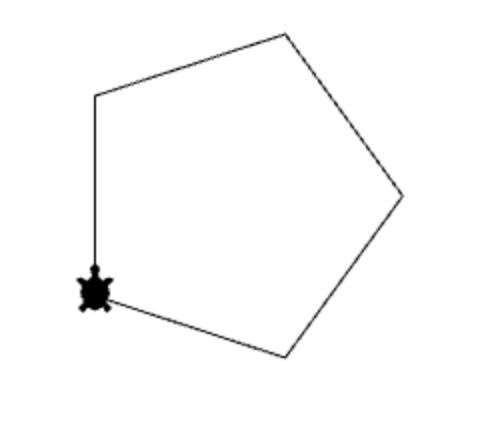
\includegraphics[width=\linewidth]{GrundlagenInfo/00_Programmieren/Figures/vieleck}
\end{figure}
\end{column}
\end{columns}
\end{frame}

\begin{frame}[fragile]{Vieleck mit Variablen, \textit{hard-coded} \emoji{pencil}}
\begin{columns}
\begin{column}{.7\textwidth}
\begin{lstlisting}
from gturtle import *
makeTurtle()

def vieleck():
    # Anzahl Ecken und Seitenlänge 
    # sind "hard-coded"
    ecken = 5
    laenge = 100
    repeat ecken:
        fd(laenge)
        rt(360/ecken)

vieleck()
\end{lstlisting}
$\rightarrow$ Kennen Sie bereits!
\end{column}
\begin{column}{.3\textwidth}
\begin{figure}
\centering
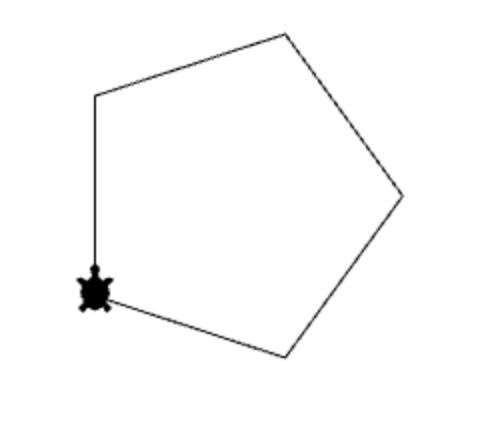
\includegraphics[width=\linewidth]{GrundlagenInfo/00_Programmieren/Figures/vieleck}
\end{figure}
\end{column}
\end{columns}
\end{frame}


\begin{frame}[fragile]{Vieleck mit Variablen, \textit{on-the-fly} \emoji{airplane}}
\begin{columns}
\begin{column}{.7\textwidth}
\begin{lstlisting}
from gturtle import *
makeTurtle()

def vieleck():
    # Anzahl Ecken und Seitenlänge 
    # mit input('...')"
    ecken = input("Wie viele Ecken?")
    laenge = input("Seitenlänge?")
    repeat ecken:
        fd(laenge)
        rt(360/ecken)

vieleck()
\end{lstlisting}
\end{column}
\begin{column}{.3\textwidth}
\begin{figure}
\centering
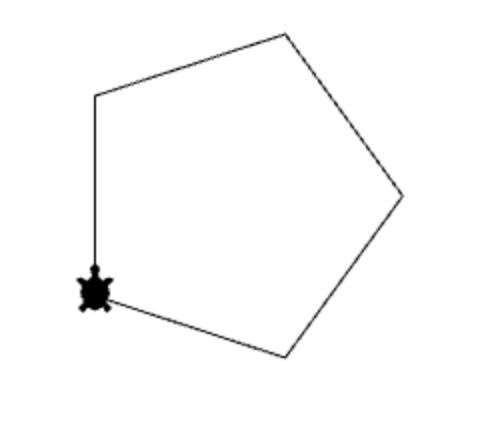
\includegraphics[width=\linewidth]{GrundlagenInfo/00_Programmieren/Figures/vieleck}
\end{figure}
\end{column}
\end{columns}
\end{frame}

\begin{frame}[fragile]{Vieleck mit Variablen, \textit{on-the-fly} \emoji{airplane}}{Nützlicheres Beispiel}
\begin{lstlisting}
from gturtle import *
makeTurtle()

def vieleck():
    # Anzahl Ecken und Seitenlänge mit input('...')"
    ecken = input("Wie viele Ecken?")
    laenge = input("Seitenlänge?")
    repeat ecken:
        fd(laenge)
        rt(360/ecken)

def mehrere_vielecke(anzahl):
    repeat anzahl:
        vieleck()

mehrere_vielecke(3)
\end{lstlisting}
$\rightarrow$ Demo
\end{frame}

\begin{frame}[fragile]{Zusammenfassung}
\begin{itemize}
\item Bei \lstinline|input| sind die Variablen-Werte vor der Programm-Ausführung \textit{unbekannt}!
\item Ermöglicht es, flexibel Variablenwerte \textit{während} der Programm-Ausführung zu definieren (\textit{on-the-fly} \emoji{airplane})
\end{itemize}
\end{frame}

\begin{frame}[fragile]{Auftrag}
\begin{itemize}
\item \abgabebox{Aufgaben 3.40, 3.42 (Moodle)}
\item \aufgabebox{Aufgabe 3.41}
\item \aufgabebox{Aufgaben 3.1, 3.2, 3.3 (am Ende des Kapitels)}
\end{itemize}
\end{frame}